\documentclass[letterpaper,man,natbib,floatsintext]{apa7}  %Leave this stuff alone

\usepackage[english]{babel}
\usepackage[utf8x]{inputenc}
\usepackage{amsmath}
\usepackage{graphicx}
\usepackage{hyperref}

\graphicspath{ {img/} }
\captionsetup{justification=centering}

\begin{document}
%Below is what you can edit
\title{The effects of difficulty and prior expertise levels in educational video games}
\shorttitle{Expertise and difficulty levels in educational video games}
\author{Shail Patel}
\affiliation{Rensselaer Polytechnic Institute}

\abstract{Video games offer a method to educate students interactively in online environments. However, the 
effectiveness of online courses can be affected by a student's preexisting knowledge of a subject. A course that is 
more guided and walks a player through every step may be preferred by inexperienced players but may be considered 
boring to more experienced players. These two knowledge groups are in conflict
with one another and a course designed around one group may alienate the other. In order to explore this difference 
in expertise, an educational video game experience has been created that can generate a course style with different 
levels of difficulty. A course is defined as a series of levels, where each level is a single problem that must be solved by the player. Players self report their prior expertise on the subject and are assigned a random difficulty level. The play-through is then measured as levels are completed. The findings show support for high expertise players  
responding more positively to challenging courses while less experienced players avoid levels considered too challenging. 
Less experienced players also have a smaller rate of course completion level which may indicate a higher level of internal
motivation with additional experience.}

\keywords{Education, gamification, computer science, learning}

\maketitle

\section{Introduction}
Computer simulations have long been used for learning and practice in various disciplines. From medicine to the military, simulations have created training environments that allow mastery over skills without needing to be exposed 
to costly or dangerous scenarios in the world. \cite{lateef2010simulation} notes the increase in simulation-based learning within the field of medicine to increase performance and reduce errors. In medicine, simulation based learning has a long history, stretching back to mannequin simulators in the 1960s as a method to ensure a proper experience without risking patient treatment. As simulations become more accessible through modern computers and smartphones, their use
in highly specialized disciplines is now becoming more widespread. In order to appeal to a more general audience, 
designs, technology, and other knowledge is being borrowed from video games which has led to the concept of ``gamification''. \cite{deterding2011game} define {\it gamification} as ``the  use  of game  design  elements  in  non-game contexts''. Concepts borrowed from video games allow for more interactive experiences, unlike other types of media, video games demand 
a person's attention to continue, unlike passive media like video or television, video games will typically not continue unless a person interacts with it. Compared to other active media, like reading, video games can also respond to a player's choices. This is ideal for a learning environment where material can be displayed to the player and tested before progressing.

As gamification becomes more popular in academia and in industry, interest in its effectiveness has grown. A literature
review of empirical studies in gamification by \cite{hamari2014does} found that many studies focus on psychological outcomes such as motivation, engagement, and fun. The study also found the gamification context and the qualities of the users were two important confounding factors that could affect outcomes. However, fewer studies focused on learning outcomes and effectiveness.

\subsection{Purpose of current study}
Understanding how gamification can become more effective is important as its adoption grows and can allow better
designed experiences for students. \cite{kalyuga2009expertise} describes the ``The Expertise Reversal Effect'' in
multimedia learning as the effect where 
instruction techniques that are effective with inexperienced learners may not be as effective for experienced learners. 
Inexperienced learners will also be less effective with more complex and less guided instructions that more 
experienced learners benefit from. The study concludes that fully guided instruction is redundant for experienced learners but essential for novice learners. As a result, gamified experiences that try and cater to all types of knowledge levels
may not be as effective those that are made for a specific audience. This presents the opportunity to use technology to
create individual experiences that can adapt to a person's knowledge level. The possibility of automatically generating
a course to users by tweaking specific parameters in a game could lead to more effective instruction while also reducing
the amount of development required to build an experience. Since fully guided instruction is more difficult to perform in
an electronic learning medium understanding if difficulty can also create an effect similar to expertise reversal is of 
interest. A review of empirical studies by \cite{kalyuga2007expertise} related to the expertise reversal effect proposes a
framework for adaptive learning environments that can be utilized in electronic learning. In their review, the study proposes learner knowledge is ``the single most important cognitive characteristic that influences learning and 
performance'' (pg 2). Although electronic and gamified experiences may be the best suited for adaptive learning 
designs, very few appear to utilize them. A literature review by \cite{majuri2018gamification} notes that many studies
focused on user factors such as personal preferences, interests, and other choices by the user that encourage them
to continue playing whereas adaptive learning appears in very few studies. As a result, there is an opportunity to
study adaptive learning in gamification contexts and how it may change effectiveness. Adaptive learning could
also have an effect on the expertise reversal effect and could be a possible intervention in preventing it from occurring
when different knowledge levels play the same game.

\section{Experiment Design}
This study was performed by creating an interactive experience about different models of computation, a topic common in 
both introductory and advanced theoretical computer science (CS) classes. The game covers Finite State Machines (FSMs), Pushdown automata (PDs),
and finally Turing Machines (TMs). Initially, participants are introduced to the interface by creating a simple FSM. This part is guided to ensure each participant knows how to solve later puzzles and how input is fed into each automaton. Each type of model of computation has its own tutorial level for users not familiar with it. Users may also open a help page
that allows them to revisit the rules and instructions at any time when playing.
Afterward, each level has a description of a certain type of problem that can be solved by an automaton. A list of inputs 
to be accepted and rejected is also displayed to the user. Figure \ref{fig:interface} below shows an example level for accepting strings with an even number of ones and rejecting otherwise. 
\begin{figure}[h!]
	\centering
	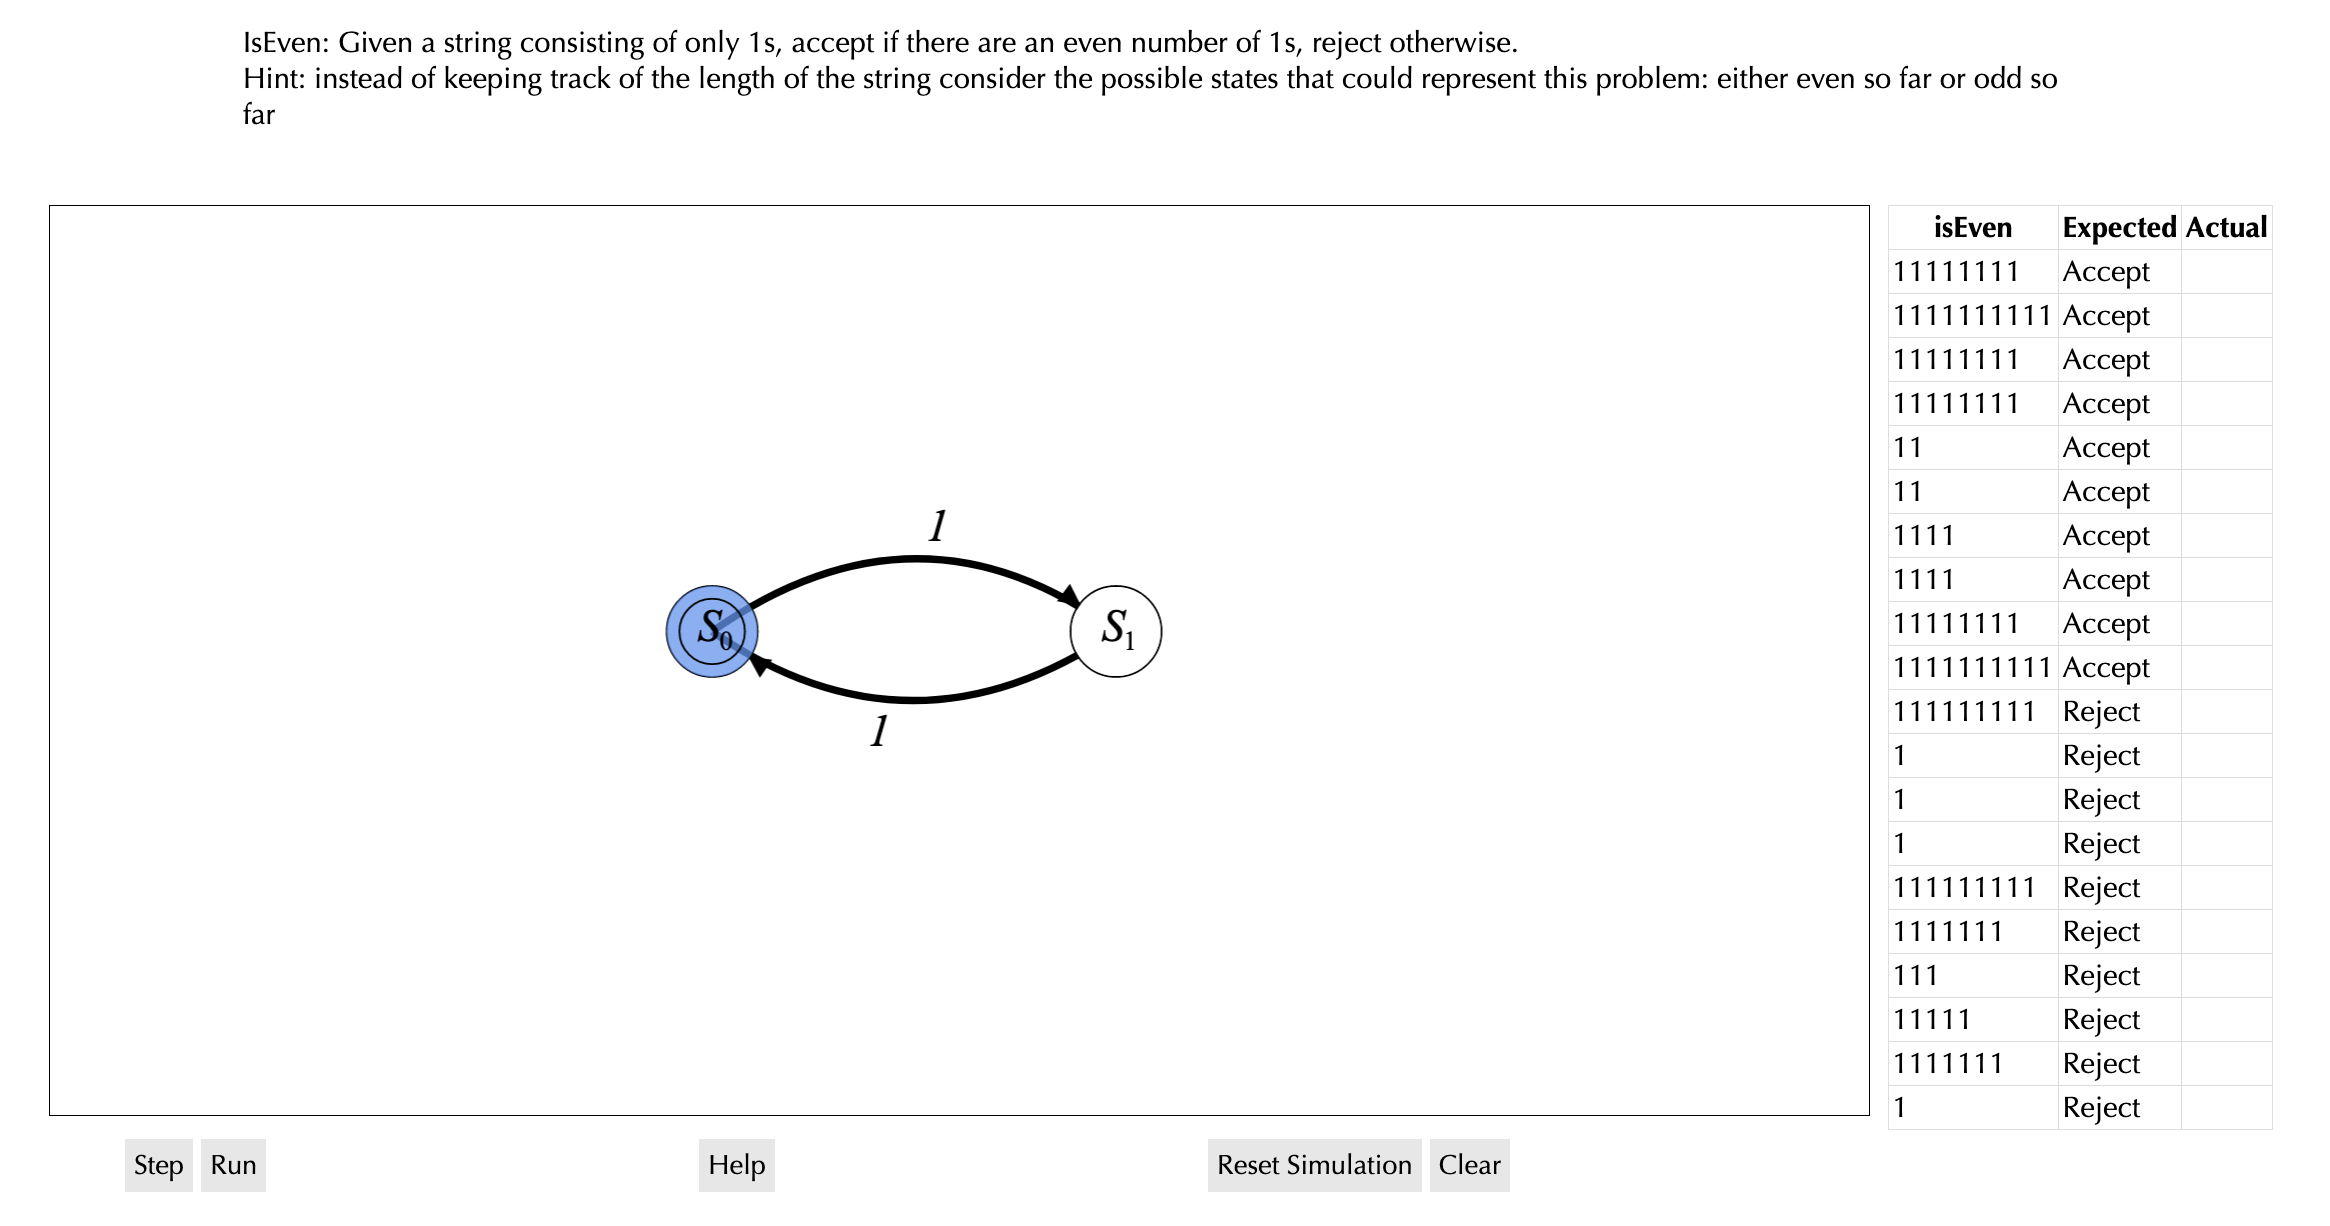
\includegraphics[width=0.9\textwidth]{example_interface_1}
	\caption{Creating a FSM using the game interface}
	\label{fig:interface}
\end{figure}
The interface can be accessed on any browser and upon first loading the user is asked for their experience with models of computation on a level from 0 to 10, 10 being very experienced and 0 having little to no prior knowledge. 
Low experience is considered responses from 0 to 3.3, medium experience as greater than 3.3 to 6.6 and high experience as greater than 6.6 to 10.
Each user is
randomly assigned into a difficulty group, either {\it easy}, {\it medium}, or {\it hard}. Different factors play into a difficulty level. A level can include variation in the description, the objective, or additional requirements to complete
the level. For example easier levels can include hints on how to solve the puzzle, whereas harder levels have additional test cases to consider. As the participants progress, the overall difficulty increases with each level solved. Anonymous
statistics on the user's playthrough are recorded with each level completed or when a user exits the program.

The game was posted to four websites under the title {\it FiniteStates}, a standalone site, Hacker News, itch.io, and Newgrounds; see Appendix for more details. itch.io and Newgrounds are websites where games, videos and other media are uploaded, submissions are typically from independent creators and has a wide audience of players. The majority of inexperienced users who participated came from these two sites. Hacker News is a news forum focused mainly on technology, 
it is hosted by the startup incubator Y combinator. Typically users from this site were more experienced with computer science topics. Finally the standalone website was hosted and students from Rensselaer Polytechnic Institute (RPI) were asked directly to visit and play 
the game whenever they had a chance. Almost all students asked had some experience with topics covered in the game. Participants could play the game at any time they wanted and could also exit early, since the experiment was done largely in a real life environment there is limited control over each participant and instead they behavior was recorded instead.

\section{Results}
Overall a total of 155 participants played the game across all four sites. Table \ref{tab:users} shows a detailed breakdown of the participants and their reported prior experience level. The majority of the users reported low experience levels from Newgrounds, this was expected due to the wide audience that visits Newgrounds, who are typically younger and would not of had the opportunity to be exposed to theoretical CS concepts. 54\% of all participants described themselves
as having low experience with models of computation, whereas 22\% of participants said they had a medium level of experience and 24\% for high level of experienced users. 
\begin{table}[h!]
	\caption{User participation breakdown over different sites and their reported prior experience}
	\label{tab:users}
	\begin{tabular}{l|ccc|c}
		\toprule
		Site & Low experience & Medium experience & High experience & Total Participants \\
		\midrule
		Newgrounds & 72 & 14 & 6 & 90\\
		Itch.io & 5 & 5 & 2 & 12\\
		HackerNews & 5 & 7 & 9 & 21\\
		Standalone Site & 2 & 9 & 21 & 32\\
		\midrule
		Total  & 84 & 35 & 38 & 155\\
		\bottomrule
	\end{tabular}
\end{table}\\
Since the experiment was deployed publicly, it was expected that 
majority of players would not be familiar with models of computation. For this reason, individual students from RPI were asked to play the game to ensure there were a sufficient level of participants with at least a medium level of experience or higher. In the final analysis 35 responses where taken from each group, the low and high experience groups were 
subsampled to ensure each group has an equal number of responses in the analysis. 

Figure \ref{fig:dist_1} shows the distribution of the number of levels completed by a user for each knowledge level. The histograms show a sharp negative trend for low experience users and levels completed $r = -0.72, p < 0.05$, there is also a negative trend for 
medium experience users $r = -0.30, p < 0.05$, and a positive trend for high experience users $r=0.54, p < 0.05$.
Figure \ref{fig:dist_2} shows a regression fit over each breakdown, users with a medium level of experience had the most variance in the number of levels completed.
\begin{figure}[h!]
	\centering
	\makebox[\textwidth]{
		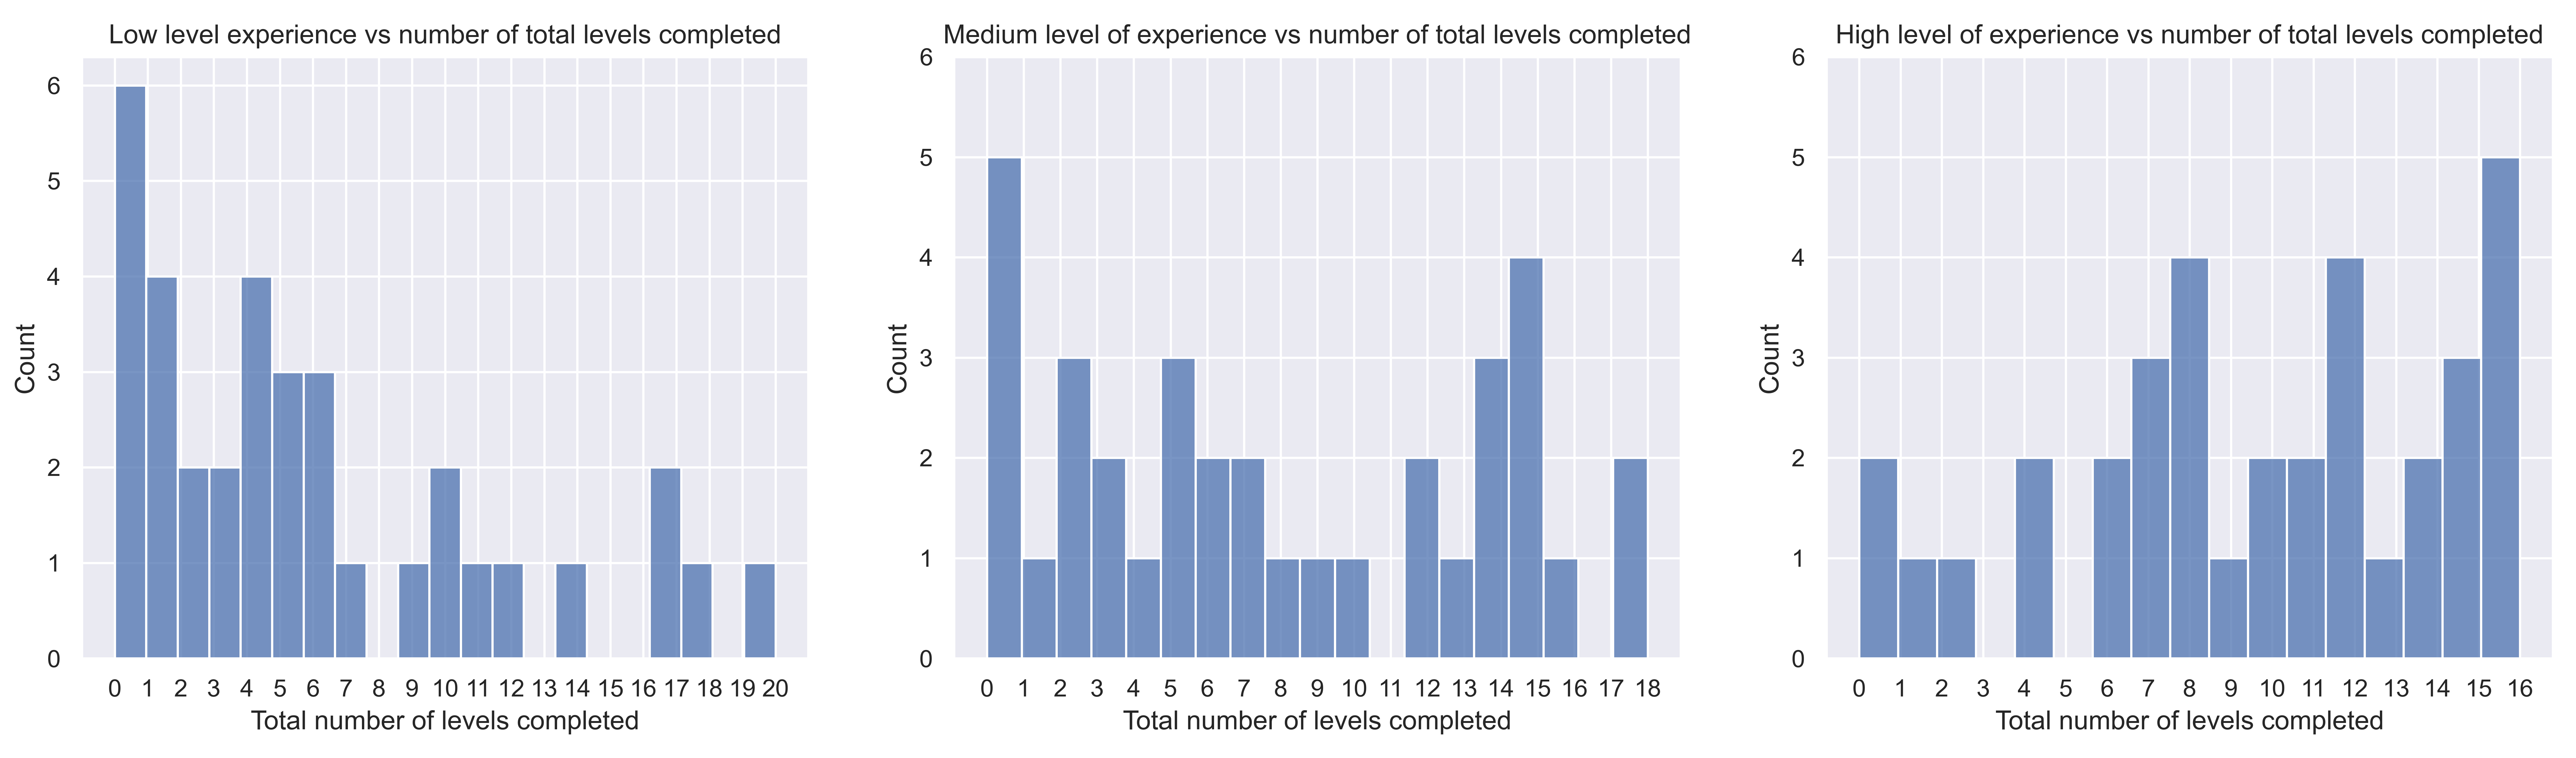
\includegraphics[width = 1.21\textwidth]{dist_1}
	}
	\caption{Distribution of number of levels completed separated by experience level}
	\label{fig:dist_1}
\end{figure}
\begin{figure}[h!]
	\centering
	\makebox[\textwidth]{
		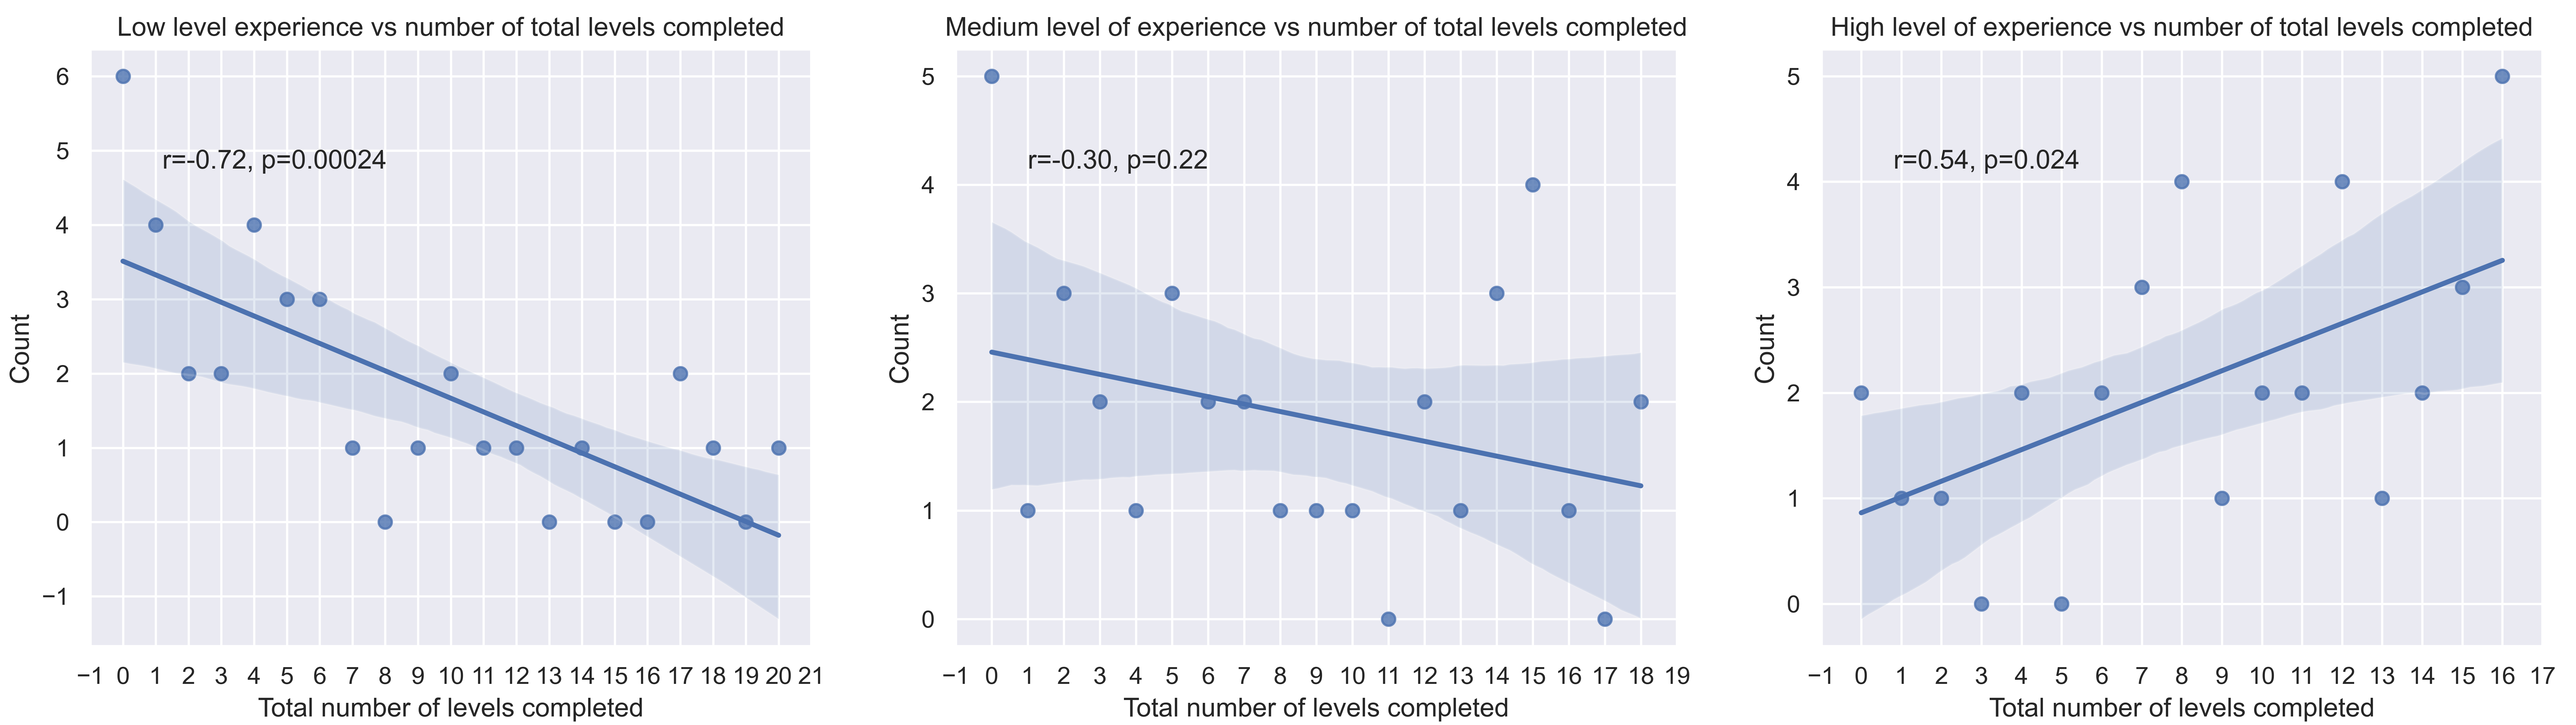
\includegraphics[width = 1.21\textwidth]{dist_2}
	}
	\caption{Regression fit for number of levels completed separated by experience level}
	\label{fig:dist_2}
\end{figure}\\
Without considering prior experience level, low experience users were far less likely to complete more levels than high experienced ones. On top of levels completed, the number of errors made per level and total time spent playing were also collected. Overall every knowledge group tended to make more mistakes at the first levels of a different model of computation and then made less over time. The number of errors made never hit zero, but instead leveled off at a low
of 5-10 per level, this is most likely from players using the interface to test different solutions, since each automaton can be simulated against different input, the mental effort of understanding the behavior of any automata is offloaded to the game.
There were no significant trends on time usage, typically highly experienced users could solve certain problems quicker, this could indicate they've seen similar puzzles before or already understand the concept being tested for the level. While 64\% of users played in a single session, a large number (34\%) of players would come back to the game in multiple sessions many hours or sometimes even days apart.

Prior knowledge appears to be a stronger indicator of levels completed compared to difficulty given, figure \ref{fig:dist_3} shows a box plot comparing responses to each variable.

High experienced users tended to respond positively to hard levels and would have high rate of level completion, and the opposite was also true. An easy difficulty would cause high experienced users to complete fewer levels. The same effect was seen in low experience users but to a smaller effect, the trend for course completion was still negative if a novice
user was given an easy difficulty or a harder one. However, the trend was less negative for when the difficulty matched
($r=-0.52, p < 0.05$). 
\begin{figure}[h!]
	\centering
	\makebox[\textwidth]{
		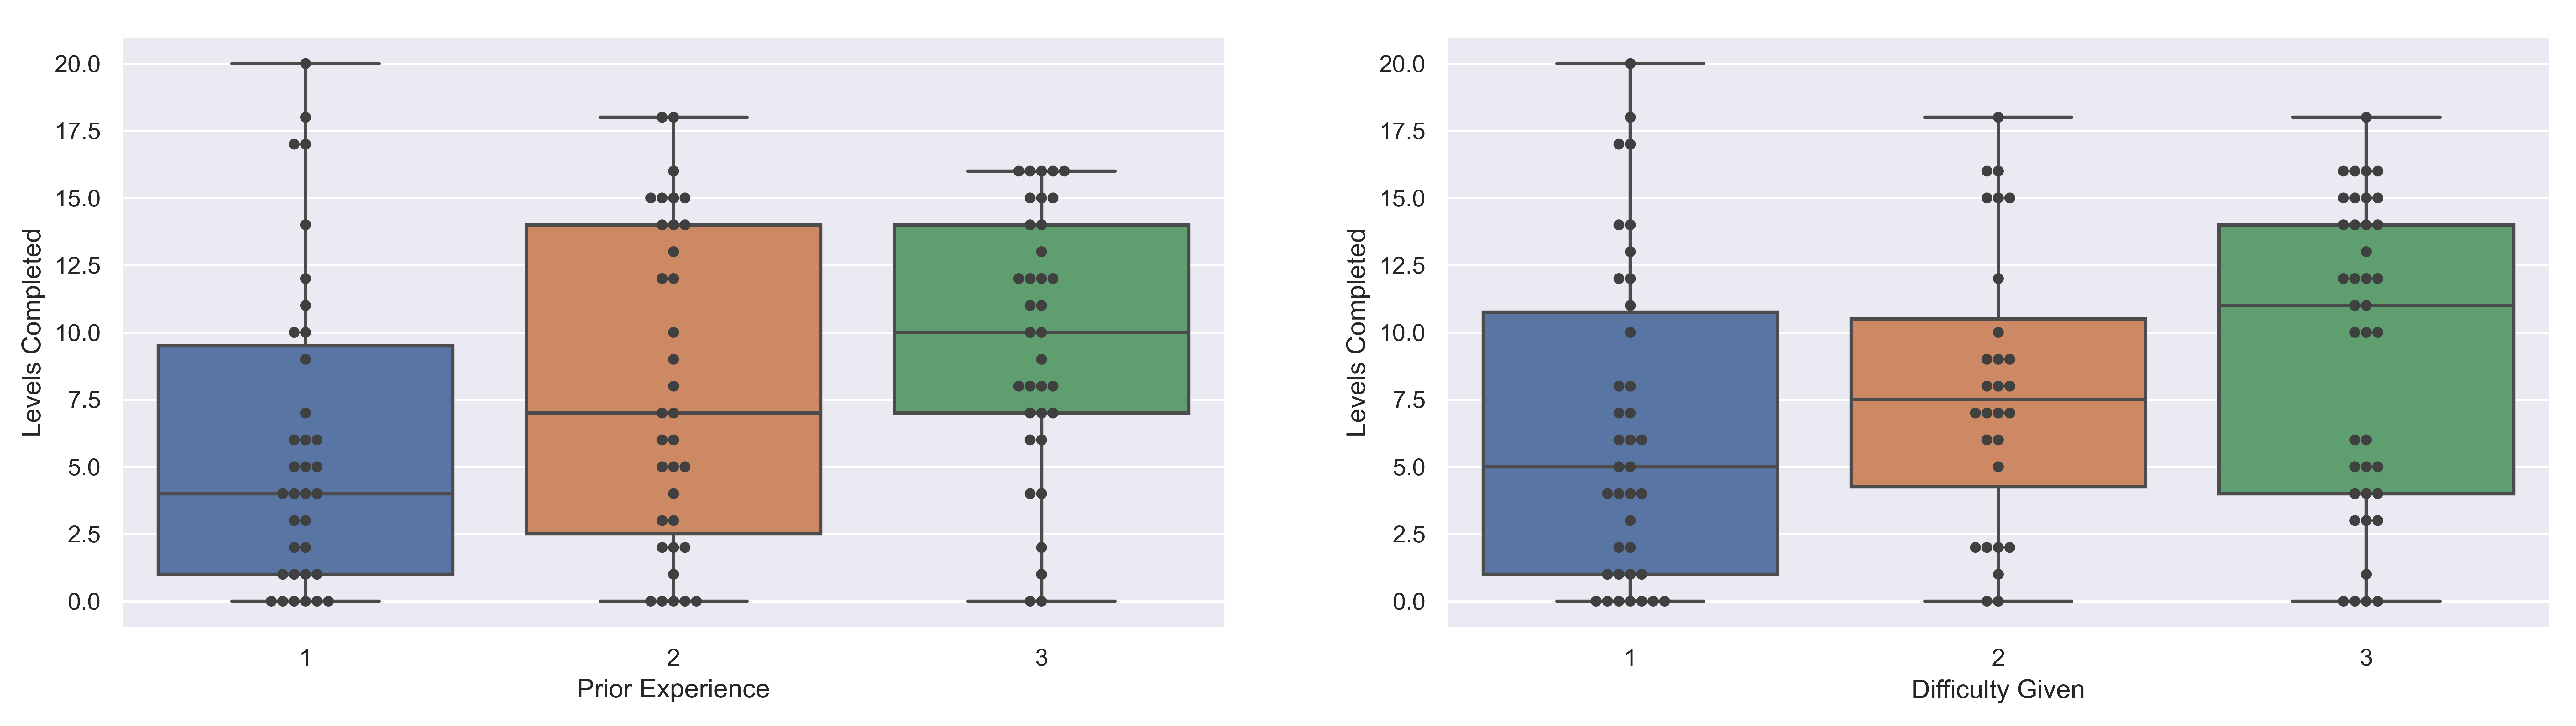
\includegraphics[width = 1.21\textwidth]{dist_3}
	}
	\caption{Box plot for responses vs Prior experience and difficulty level given}
	\label{fig:dist_3}
\end{figure}\\
There may be other factors driving the rate of course completion for novice players that have a
stronger effect than difficulty.
There is also a slight increase in the probability of a person increasing a level if they are given a hard level vs an easy level. This difference is most likely from the large difference between low and high experience players who have almost opposite
level completion rates.
\section{Discussion}
The results show that high experienced players have a higher rate of course completion than other knowledge groups 
which only increases when given challenging puzzles. This could imply a higher level of internal motivation that allows
them to continue progressing whereas less experienced players may need additional reasons to keep playing that other game features would have to compensate for. Medium and low experience players had a worse rate of course completion but medium experience players had a positive trend when given a difficulty level that matched their prior experience but low experience still had a negative trend, although less negative than when not considering difficulty level given. These results show a weaker effect that is similar to the expertise reversal effect but one that is less visible in novice 
players.

Although the courses generated for each user were generated randomly at the start, when each player was given a difficultly level, the ability for the game to adapt to the players is very possible. By tracking the number of errors made and the time taken per level, and potentially other indicators in the future it would be possible to dynamically 
judge the player's current knowledge level and adjust the difficulty to instruct more effectively. In this experience 
the puzzles were open ended but perhaps adding more guided components would have increased the number of levels completed
by novice players. After completing the introduction, players are thrown into a puzzle which may be too steep of a learning curve and newer players would prefer a guided section stretched over multiple levels before given one to solve on their own. Although this paper studies different gamification contexts, the experience created is closer to a simulation then game due to lack of actual game features. This could be an additional reason for the high number of novice
players that did not complete any level after finishing the introduction. In the reviews mentioned earlier some of the most common gamified features are a leaderboard of scores or statistics for users, a narrative, and rewards for progress which could be implemented in the future to see any difference in level completion. The experience was also deployed publicly on sites that have hundreds of other options and users may simply decide their time is better spent on something else.

Although learning in this study is simply measured by proxy to the number of levels completed it is difficult to measure learning directly. For example it is not clear how students may perform on exams relating to the material if they 
played the game first. Many users continue to make some level of mistakes even in later puzzles which suggests they 
are offloading the cognitive load of knowing how automata may work to the game itself since they can quickly 
try different combinations and simulate it to see its effects. As a result, users may have a greater level of
understanding but may not be able to understand how an automaton may process specific input without the help of software, although this hypothesis is untested.
\subsection{Limitations of the Study}
The largest limitations come from the decision to perform the experiment in the field than from a laboratory setting. Since the player data is anonymous there is no way to know the background of a user without asking them further questions through the game itself. Currently the method chosen the gauge the prior knowledge of a user was to ask them to self report on a 0 to 10 scale which is difficult to describe a person's entire knowledge over a single number. The idea of being a novice at a subject verses being an expert at it can also vary between person too. Novice users are more likely to self report a higher level of understanding than they may actually have \cite{kruger1999unskilled}. Users were also free to either stop playing at any time or play the game in multiple sessions, this was done since it was difficult to control for, however there may be some effect on the results by the group of users that decided to play in multiple sessions. Students who were personally asked to play the game may of had a higher level of motivation to complete more levels then those discovering the game online and volunteering to play, however, all users when asked where explicitly 
told they only had to play as much as they wanted and could stop whenever they like. Regardless there is more likely a higher level of course completion from those asked to play and if this experiment was recreated in laboratory conditions, the overall completion rate would most likely be higher based on participant expectations. On first visiting the game, 
users would be given a unique identifier based on random characters as an ID. This ID is browser specific and could be cleared if a browser's history is erased so there is a possibility of users playing the game multiple times on either different browsers or after their first save data has been wiped although its hard to see any evidence for this.
\subsection{Advantages of the study}
There are advantages to the field experiment setup, the biggest being a more realistic environment that collects a broader range of participants. For example, \cite{henrich2010weirdest} notes that the majority psychological studies (67\%)
use undergraduate students with a background in psychology for studies that typically generalize across the entire population. By opening up participants to anyone online, the range of backgrounds that are tested is dramatically expanded, although in this scenario its not possible to see those different backgrounds and of course certain audiences are more likely to visit specific sites over others as mentioned earlier. Since the experiment is largely automated, it
can also be reproduced easier. The code is open source on GitHub and can be deployed again to other sites. By being able 
to run the game in a desktop browser, any modern computer can access it without the user needing to download any software
beforehand which could be a barrier to entry. Since the game is played in a browser users would typically have internet access for statistics to be recorded as they played. All of the statistics collected are anonymous and cannot be used to 
track the user. The separation between the user and any researcher prevents any issues from the experiment implementation 
since the software and user are responsible and a researcher would only be able to see statistics after the user is 
finished playing.

\subsection{Conclusion}
This study confirms the importance of prior knowledge in the effectiveness of learning found in other studies and 
specifically in the context of gamification is an underutilized tool that may be creating ineffective learning tools 
for certain students. Expert players have a higher level of internal motivation and require fewer mechanics to 
encourage progression compared to novice players. Using a difficulty level that is not preferred by a knowledge group  has some effect similar to the expertise reversal effect whereas using the desired difficulty level may mitigate 
the expertise reversal effect in certain knowledge groups.

\appendix{
\section{Sites used in experiment}
	%\begin{itemize}
	   \indent 
	   \indent \href{https://www.newgrounds.com/}{Newgrounds}\\
	   \href{https://news.ycombinator.com/}{Hacker News}*\\
	   \href{http://itch.io/}{itch.io}\\
	   \href{shailpatels.me/FiniteStates/}{Standalone Site}\\~\\
	%\end{itemize}
}
\noindent
* Since HackerNews is a forum and doesn't host content itself, a separate site was created that had its 
results marked with an indicator to denote a user was from HackerNews. The game is still playable in the standalone site, the status of other sites may change.

\bibliography{Bibliography}

\end{document}
